The agenda for this section is as follows. In \sref{parameters}, the uncertain
parameters $\vu$ are transformed into a form suitable for the subsequent
calculations. This stage is an essential part of our framework. The rest of the
subsections, \sref{time}, \sref{power}, and \sref{temperature}, serve a strictly
illustrative purpose. They introduce a number of models and a number of
quantities of interest $\g$ in order to give the reader a better intuition about
the utility of the framework. These models and quantities also give us concrete
problems to work with in the section on experimental results,
\sref{experimentation}. It should be well understood that the essence of $\g$ is
problem specific. Therefore, the exact formulation of $\g$ is left to the
designer's discretion.

\subsection{Uncertainty Parameters} \slab{parameters}
The foremost step of our framework is to change the parameterization of the
problem from the random vector $\vu = (\u_i)_{i = 1}^\nu \sim \distribution_\vu$
to an auxiliary random vector $\vz = (\z_i)_{i = 1}^\nz \sim \distribution_\vz$
such that: 1) the support of $\distribution_\vz$ is the unit hypercube $[0,
1]^\nz$, and 2) $\nz \leq \nu$ has the smallest value needed to retain the
desired level of accuracy. The first is standardization, which is done primarily
for convenience. The second is model-order reduction, which identifies and
eliminates excessive complexity and, hence, speeds up the solution process. The
reduction is possible whenever there are dependencies between $(\u_i)_{i =
1}^\nu$, in which case one can find such $(\z_i)_{i = 1}^\nz$, $\nz < \nu$, that
each $\u_i$ can be recovered from $(\z_i)_{i = 1}^\nz$. We shall denote the
overall transformation by $\vu = \transformation(\vz)$ where
\begin{equation} \elab{transformation}
  \transformation: \real^\nu \to [0, 1]^\nz.
\end{equation}
For any point $\vz \in [0, 1]^\nz$, we are now able to compute the corresponding
$\vu$ and, consequently, the quantity of interest $\g$ as $(\g \circ
\transformation)(\vz) = \g(\transformation(\vz)) = \g(\vu)$; recall also
\sref{problem}.

Let us consider an example of $\transformation$ in order to understand the
concept better. To this end, we begin by assuming that the distribution of $\vu
= (\u_i)_{i = 1}^\nu$, $\distribution_\vu$, is given as a set of marginal
distribution functions $\{ \distribution_{\u_i} \}_{i = 1}^\nu$ and a copula
\cite{nelsen2006} (see also \sref{preliminaries}). Furthermore, the copula is
assumed to be a Gaussian copula whose correlation matrix is $\correlation \in
\real^{\nu \times \nu}$.

\begin{remark}
A set of marginals and a copula entirely characterize the joint distribution of
$\vu$, that is, $\distribution_\vu$. However, we consider this distribution as
an approximation rather than as the true one. The knowledge of the true joint
would be an impractical assumption to make. A more realistic assumption is the
availability of the marginals and correlation matrix of $\vu$. In general, these
two pieces are not sufficient to recover the joint of $\vu$; however, the joint
can be approximated well by accompanying the available marginals by a Gaussian
copula constructed based on the available correlation matrix; see \cite{liu1986}
and also \cite{ukhov2014}. Hence, a set of marginals and a Gaussian copula are
practical inputs to probabilistic analysis.
\end{remark}

The number of variables, which is so far $\nu$, has a significant impact on the
complexity of the problem at hand. Therefore, an important component of our
framework is model-order reduction, which we shall base on the discrete
Karhunen--Lo\`{e}ve decomposition, also known as the principal component
analysis. We proceed as follows. Since any correlation matrix is real and
symmetric, $\correlation$ admits the eigendecomposition: $\correlation = \m{V}
\m{\Lambda} \m{V}^T$ where $\m{V} \in \real^{\nu \times \nu}$ is an orthogonal
matrix whose columns are the eigenvectors of $\correlation$, and $\m{\Lambda} =
\diag(\lambda_i)_{i = 1}^\nu$ is a diagonal matrix whose diagonal elements are
the eigenvalues of $\correlation$. The eigenvalues $(\lambda_i)_{i = 1}^\nu$
correspond to the variances of the corresponding components revealed by the
decomposition. The model-order reduction boils down to selecting those major
components whose cumulative contributions to the total variance is above a
certain threshold. Formally, assuming that $(\lambda_i)_{i = 1}^\nu$ are sorted
in the descending order and given a threshold $\eta \in (0, 1]$ specifying the
fraction of the total variance to be preserved, we identify the smallest $\nz$
such that
\begin{equation} \elab{reduction}
  \frac{\sum_{i = 1}^\nz \lambda_i}{\sum_{i = 1}^\nu \lambda_i} \geq \eta.
\end{equation}
Denote by $\tilde{\m{V}} \in \real^{\nu \times \nz}$ and $\tilde{\m{\Lambda}}
\in\real^{\nz \times \nz}$ the matrices obtained by truncating $\m{V}$ and
$\m{\Lambda}$, respectively, to preserve only the first $\nz$ components where
$\nz$ is as shown above.

Now, the transformation $\transformation$ in \eref{transformation} is
\begin{equation} \elab{transformation-concrete}
  \vu = \distribution_\vu^{-1} \left( \Phi\left( \tilde{\m{V}} \tilde{\m{\Lambda}}^\frac{1}{2} \, \Phi^{-1}(\vz) \right) \right)
\end{equation}
where the \rvs\ $\vz = (\z_i)_{i = 1}^\nz$ are independent and uniformly
distributed on $[0, 1]^\nz$; $\Phi$ and $\Phi^{-1}$ are the distribution
function of the standard Gaussian distribution and its inverse, respectively,
which are applied elementwise; and $\distribution_\vu^{-1} =
\distribution_{\u_1}^{-1} \times \cdots \times \distribution_{\u_\nz}^{-1}$ is
the Cartesian product of the inverse marginal distributions of $\vu$, which are
applied to the corresponding element of the vector yielded by $\Phi$. In the
absence of correlations, \eref{transformation-concrete} is simply $\vu =
\distribution_\vu^{-1}(\vz)$, and no model-order reduction is possible ($\nu =
\nz$). It might be interesting to note that, using the above transformation, the
distribution $\vu$ gets ``baked'' in $\g$ because it ``disappears'' when $\g$ is
viewed as a function of $\vz$, distributed uniformly.

To summarize, we have found such a transformation $\transformation$ and the
corresponding random vector $\vz \sim \distribution_\vz$ that: 1)
$\distribution_\vz$ is supported by $[0, 1]^\nz$, and 2) $\vz$ has the smallest
number of dimensions $\nz$ needed to preserve $\eta$ portion of the variance.


\begin{figure*}
  \centering
  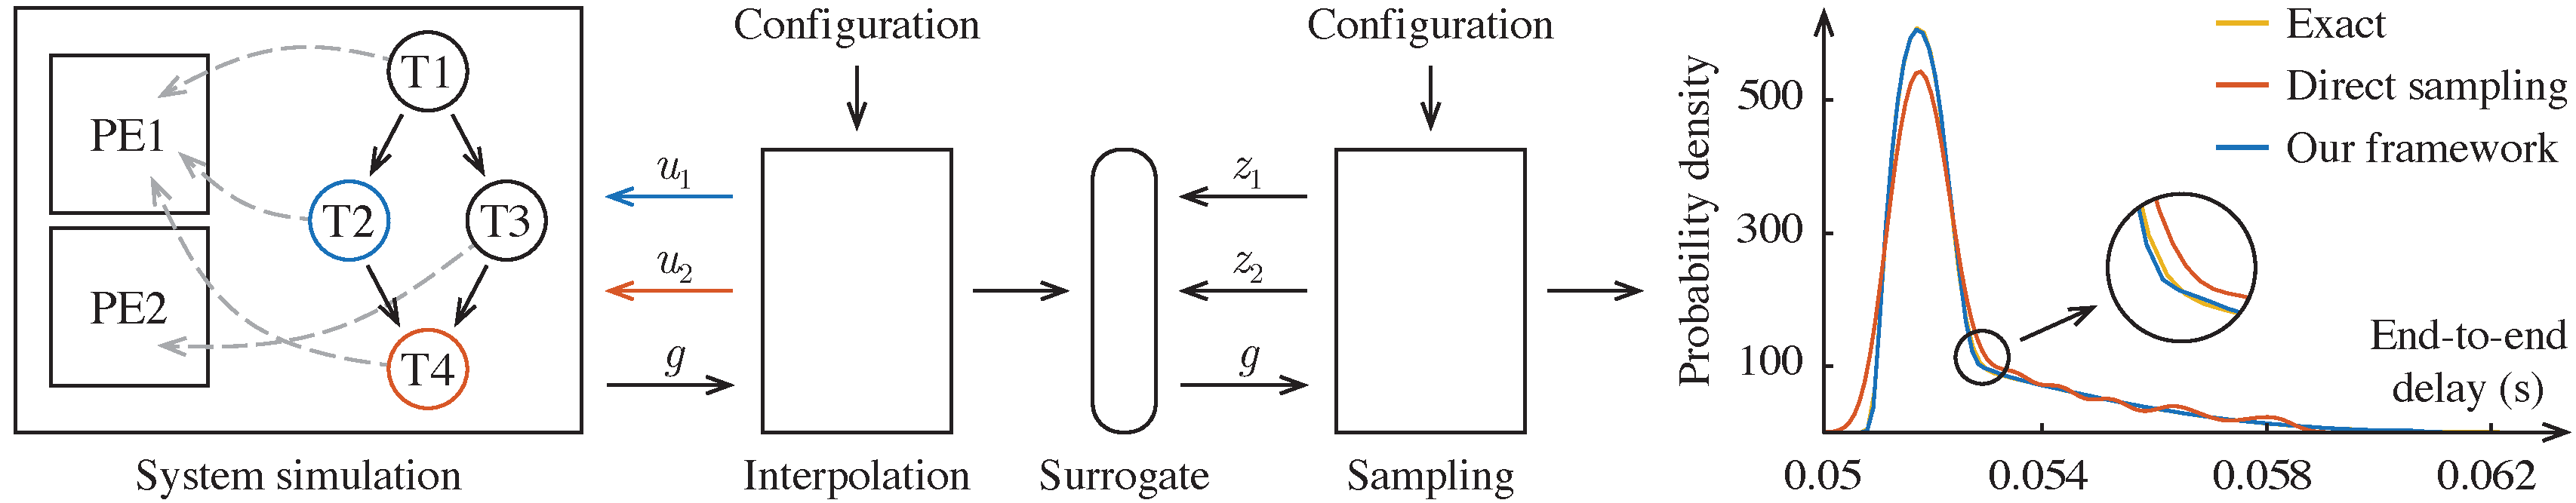
\includegraphics[width=1.0\textwidth]{include/assets/figures/example.pdf}
  \vspace{-1.5em}
  \caption{
    The proposed framework applied to analyze the end-to-end delay of an
    application whose two out of four tasks have random execution times.
  }
  \flab{example}
  \vspace{-1em}
\end{figure*}

\subsection{Application Timing} \slab{time}
Suppose the application is given as a directed acyclic graph. The vertices
represent tasks, and the edges data dependency between these tasks. Suppose
further that a static cyclic scheduling policy is utilized. Note, however, these
assumptions are orthogonal to our framework: the framework can be applied to any
application model and any scheduling policy.

Each task has a start and a finish time. For task $i$, denote these two time
moments by $\b_i$ and $\d_i$, respectively, and let $\vb = (\b_i)_{i=1}^\nt$ and
$\vd = (\d_i)_{i=1}^\nt$. Other timing characteristics of the application can be
derived from $(\vb, \vd)$. An example is the end-to-end delay, which is the
difference between the finish time of the latest task and the start time of the
earliest task:
\begin{equation} \elab{end-to-end-delay}
  \text{End-to-end delay} = \max_{i = 1}^\nt \, \d_i - \min_{i = 1}^\nt \, \b_i.
\end{equation}

Suppose the execution times of the tasks depend on $\vu$ (see \sref{problem}).
Then the tuple $(\vb, \vd)$ depends on $\vu$. \updated{Then the end-to-end delay
given in \eref{end-to-end-delay} depends on $\vu$ and is a potential metric
$\g$; it is used in \fref{example}.} Note that this $\g$ is nondifferentiable as
the $\max$ and $\min$ functions are such. Hence, $\g$ is nonsmooth, which
renders \up{PC} expansions and similar techniques inadequate for this problem,
as illustrated in \sref{introduction}.

\begin{remark} \rlab{smoothness}
In general, the behavior of $\g$ with respect to continuity, differentiability,
and smoothness cannot be inferred from the behavior of $\vu$. Even when the
parameters are perfectly behaved, $\g$ can still and likely will exhibit
nondifferentiability or even discontinuity, which depends on how $\g$ works
internally. For example, as shown in \cite{tanasa2015}, even if execution times
of tasks are continuous, due to the actual scheduling policy, end-to-end delays
are very often discontinuous.
\end{remark}


\subsection{Power Consumption} \slab{power}
Denote the number of processing elements present on the platform by $\np$. Let
the dynamic power consumed by task $j$ when running on processing element $i$ be
fixed during the execution of the task and denote this dynamic power by
$\p^\dynamic_{ij}$. The fact that $\p^\dynamic_{ij}$ is constant might seem
restrictive. However, one should keep in mind that it is an example. Our
framework does not have such a restriction. Even in this simple model, the
modeling accuracy can be substantially improved by representing large tasks as
sequences of smaller tasks.

Let the vector $\vp(\t) = (\p_i(\t))_{i = 1}^{\np}$ capture the total power
consumption of the system at time $\t$. This vector is related to the dynamic
power introduced above as follows:
\begin{equation} \elab{power}
  \p_i(\t) = \sum_{j = 1}^\nt \p^\dynamic_{ij} \: \delta_{ij} (\t) + \p^\static_i(\t), \hspace{1em} \text{for $i = 1, \dots, \np$},
\end{equation}
where $\delta_{ij}(\t)$ is an indicator function (outputs either zero or one) of
the event that processing element $i$ executes task $j$ at time $\t$, and
$\p^\static_i(\t)$ is the static power consumed by processing element $j$ at
time $\t$. The last component depends on time because the leakage power and
temperature are interdependent \cite{liu2007}, and temperature changes over time
(see the next subsection).

Given a set of $\ns$ points on the timeline $\{ \t_i \}_{i = 1}^\ns$,
\eref{power} can be used to construct a power profile of the system as follows:
\[
  \mP = (\p_i(\t_j))_{i = 1, j = 1}^{\np, \ns} \in \real^{\np \times \ns}.
\]
The above is a matrix where row $i$ captures the power consumed by processing
element $i$ at the $\ns$ time moments.

The total energy consumed by the system during an application run can be
computed by integrating \eref{power} over the time span of the
application---which is demarcated by the minuend and subtrahend in
\eref{end-to-end-delay}---and the corresponding integral can be estimated using
the power profile as follows:
\begin{equation} \elab{total-energy}
  \text{Total energy} = \sum_{i = 1}^\np \int \p_i(\t) \, \d\t \approx \sum_{i = 1}^\np \sum_{j = 1}^\ns \p_i(\t_j) \, \Delta\t_j
\end{equation}
where $\Delta\t_j$ is either $\t_j - \t_{j - 1}$ or $\t_{j + 1} - \t_j$,
depending on how power values are encoded in $\mP$. The assumption that
\eref{total-energy} is based on is that each $\Delta\t_i$ is sufficiently small
so that the power consumed within the interval does not change significantly.

Since the tuple $(\vb, \vd)$ depends on $\vu$, the power consumption of the
system depends on $\vu$ too. Consequently, the total energy given in
\eref{total-energy} depends on $\vu$ and is a candidate for $\g$. Note that
\rref{smoothness} applies in this context to the full extent.


\subsection{Heat Dissipation} \slab{temperature}
Based on the specification of the platform including its thermal package, an
equivalent thermal \up{RC} circuit is constructed \cite{skadron2004}. The
circuit comprises $\nn$ thermal nodes, and its structure depends on the intended
level of granularity, which impacts the resulting accuracy. For clarity, we
assume that each processing element is mapped onto one corresponding node, and
the thermal package is represented as a set of additional nodes.

The thermal dynamics of the system are modeled using the following system of
differential-algebraic equations \cite{ukhov2014, ukhov2012}:
\begin{subnumcases}{\elab{thermal-system}}
  \mC \frac{\d\vs(\t)}{\d\t} + \mG \vs(\t) = \mM \vp(\t) \\
  \vq(\t) = \mM^T \vs(\t) + \vq_\ambient
\end{subnumcases}
The coefficients $\mC \in \real^{\nn \times \nn}$ and $\mG \in \real^{\nn \times
\nn}$ are a diagonal matrix of thermal capacitance and a symmetric,
positive-definite matrix of thermal conductance, respectively. The vectors
$\vp(\t) \in \real^\np$,  $\vq(\t) \in \real^\np$, and $\vs(\t) \in \real^\nn$
correspond the system's power, temperature, and internal state at time $\t$,
respectively. The vector $\vq_\ambient \in \real^\np$ contains the ambient
temperature. The matrix $\mM \in \real^{\nn \times \np}$ is a mapping that
distributes the power consumption of the processing elements across the thermal
nodes; without loss of generality, $\mM$ is a rectangular diagonal matrix whose
diagonal elements are equal to one.

Given a set of $\ns$ points on the timeline $\{ \t_i \}_{i = 1}^\ns$,
\eref{thermal-system} can be used to compute a temperature profile of the system
as follows:
\begin{equation*}
  \mQ = (\q_i(\t_j))_{i = 1, j = 1}^{\np, \ns} \in \real^{\np \times \ns}.
\end{equation*}
Then the maximum temperature of the system can be estimated using the
temperature profile as follows:
\begin{equation} \elab{maximum-temperature}
  \text{Max temperature} = \max_{i = 1}^\np \, \sup_{\t} \, \q_i(\t) \approx \max_{i = 1}^\np \max_{j = 1}^\ns \, \q_i(\t_j).
\end{equation}

Since the power consumption of the system is affected by $\vu$ (see
\sref{power}), the system's temperature is affected by $\vu$ as well.
\updated{Therefore, the temperature in \eref{maximum-temperature} can be
considered as a metric $\g$. Note that, due to the maximization involved, the
metric is nondifferentiable and, hence, cannot be adequately addressed using
polynomial approximations, specially taking into account the concern in
\rref{smoothness}.}


To sum up, we have discussed the transformation that needs to be applied to
$\vu$ prior to the interpolation of $\g$. We have also covered three facets of
electronic systems, namely, timing, power, and temperature, and introduced a
number of quantities of interest associated with them; we will come back to
these quantities in the section on experimental results, \sref{experimentation}.

Before we move on to interpolation, let us take a moment and apply the proposed
framework to a small problem in order to get a better feel for how all the
pieces of the framework fit together. A detailed description of our experimental
setup is given in \sref{configuration}; here we give only the bare minimum.

\newcommand{\cores}{\token{PE1} and \token{PE2}}
\newcommand{\tasks}{\token{T1}--\token{T4}}
The addressed problem is depicted in \fref{example}. We consider a platform with
two homogeneous processing elements, \cores, and an application with four tasks,
\tasks. The data dependencies between \tasks\ and their mapping onto \cores\ can
be seen in \fref{example}. \updated{This delay is also our metric $\g$.} The
uncertain parameters are the execution times of \token{T2} and \token{T4}
denoted by $\u_1$ and $\u_2$, respectively; the parameters are correlated, and
their marginal distributions are beta distributions. The (deterministic)
execution time of \token{T3} lies in the range of possible values of the
execution time of \token{T2}, which curtails the impact of $\u_1$ on $\g$ and,
thereby, makes $\g$ nondifferentiable at a certain point; see \rref{smoothness}.

The leftmost box in \fref{example} represents a simulator of the system. It
takes an assignment of the execution times of \token{T2} and \token{T3}, $\u_1$
and $\u_2$, and outputs the calculated end-to-end delay. The second box
corresponds to the transformation $\transformation$ described in
\sref{parameters}. It converts the auxiliary variables $\z_1$ and $\z_2$ into
$\u_1$ and $\u_2$ in accordance with $\u_1$ and $\u_2$'s joint distribution. The
third box is our interpolation engine (to be discussed in \sref{interpolation}).
Using 156 strategic invocations of the simulator, the interpolation engine
yields a light surrogate for the simulator (the slim box with rounded corners).
Having obtained such a surrogate, one proceeds to sampling extensively the
surrogate via a sampling method of choice (the rightmost box). The surrogate
takes $\z_1$ and $\z_2$ and returns an approximation of $\g$ at that point.
Recall that the computation cost of this extensive sampling is negligible as
$\g$ is not involved. The samples are then used to compute an estimate of the
distribution of $\g$.

In the graph on the right-hand side of \fref{example}, the blue line shows the
probability density function of $\g$ computed by applying kernel density
estimation to the samples obtained from our surrogate. The yellow line (barely
visible behind the blue line) shows the true density of $\g$; its calculation is
explained in \sref{experimentation}. It can be seen that our solution closely
matches the exact one. In addition, the orange line shows the estimation that
one would get if one sampled $\g$ directly 156 times and used only those samples
in order to calculate the density of $\g$. We see that, for the same budget of
simulations, the solution delivered by our framework is substantially closer to
the true one than the one delivered by na\"{i}ve sampling.

